\title{Data Mining - Aufgabenblatt 1}
\author{Andra Herta, Tobias Dreher}
\date{07.12.2011}

\documentclass[%
	pdftex,%              PDFTex verwenden da wir ausschliesslich ein PDF erzeugen.
	oneside,%             Einseitiger Druck.
	12pt,%                Grosse Schrift, besser geeignet für A4.
	parskip=half,%        Halbe Zeile Abstand zwischen Absätzen.
	headsepline,%         Linie nach Kopfzeile.
	footsepline,%         Linie vor Fusszeile.
	bibtotocnumbered,%    Literaturverzeichnis im Inhaltsverzeichnis nummeriert einfügen
]{scrartcl}

\usepackage[utf8]{inputenc}
\usepackage[T1]{fontenc}
\usepackage[ngerman]{babel}

\usepackage{amsmath}
\usepackage{amssymb}

\usepackage{libertine}

\usepackage{graphicx}

\usepackage{placeins}
 

\begin{document}
\maketitle

\section*{Aufgabe 1}

\begin{table}[htb]
  \centering
  \begin{tabular}{c|c|c}
    \textbf{Zahl} & \textbf{Absolute Häufigkeit} & \textbf{Relative Häufigkeit}\\
    \hline
    0 & 2 & 0,04\\
    1 & 6 & 0,12\\
    2 & 5 & 0,10\\
    3 & 9 & 0,18\\
    4 & 13 & 0,26\\
    5 & 7 & 0,14\\
    6 & 5 & 0,10\\
    7 & 3 & 0,06\\
  \end{tabular}
  \caption{Häufigkeitstabelle}
\end{table}

\begin{figure}[h]
  \begin{minipage}[b]{0.5\linewidth}
    \centering
    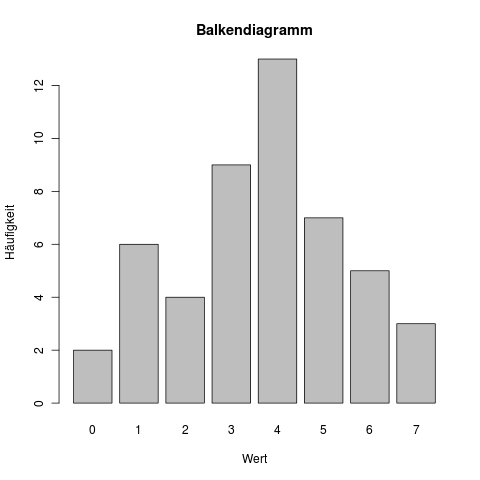
\includegraphics[width=1\linewidth]{balkendiagramm.png}
  \end{minipage}
  \begin{minipage}[b]{0.5\linewidth}
    \centering
    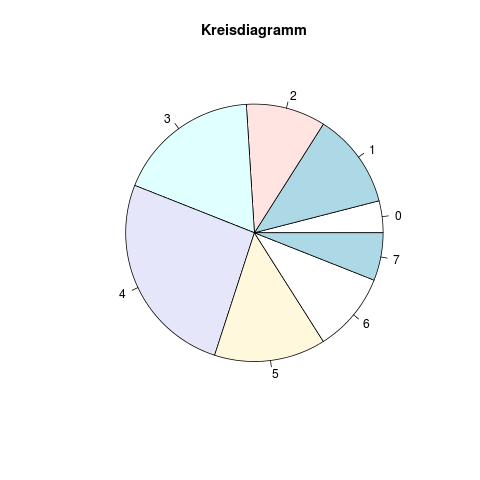
\includegraphics[width=1\linewidth]{kreisdiagramm.png}	
  \end{minipage}
\end{figure}

\FloatBarrier
\section*{Aufgabe 2}
Modalwert: $4$

Median: $\tilde{x} = 4$

1/5-Quantil: $\tilde{x}_{\frac{1}{5}} = 2$

Arithmetischer Mittelwert: $\bar{x} = 3,653061$

Spannweite: $R = 7$

Interquartilbereich: $Q := 2$

Varianz: $s^{2} = 3.314626$

Standardabweichung: $s = 1.820611$

\begin{figure}[h]
\centering
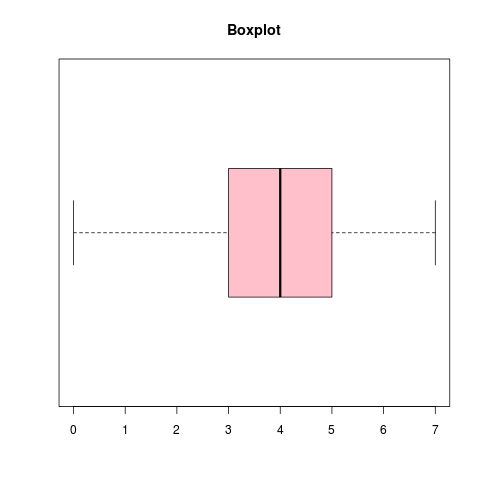
\includegraphics[width=0.55\textwidth]{boxplot.png}
\end{figure}

\FloatBarrier
\section*{Aufgabe 3}
Korrelationskoeffizient $r_{xy}$: -0.860932

\FloatBarrier
\section*{Aufgabe 4.1}
Beweis durch Causchy-Schwarzsche Ungleichung
\begin{equation}
|a \: b| \le |a| \: |b|
\end{equation}

\section*{Aufgabe 4.2}
Wenn \begin{math} y_{i} = ax_{i} + b\end{math} gilt, gilt auch \begin{math} \bar{y} = a\bar{x} + b\end{math}

\begin{equation}
r_{XY} = \frac{\sum_{i=1}^{n} (x_{i} - \bar{x}) \: (y_{i} - \bar{y})}{\sqrt{\sum_{i=1}^{n} (x_{i} - \bar{x})^{2}} \: \sqrt{\sum_{i=1}^{n} (y_{i} - \bar{y})^{2}}} 
\end{equation}

\begin{equation}
r_{XY} = \frac{\sum_{i=1}^{n} (x_{i} - \bar{x}) \: (ax_{i} + b - (a\bar{x} + b))}{\sqrt{\sum_{i=1}^{n} (x_{i} - \bar{x})^{2}} \: \sqrt{\sum_{i=1}^{n} (ax_{i} + b - (a\bar{x} + b))^{2}}} 
\end{equation}

\begin{equation}
r_{XY} = \frac{\sum_{i=1}^{n} (x_{i} - \bar{x}) \: (ax_{i} - a\bar{x})}{\sqrt{\sum_{i=1}^{n} (x_{i} - \bar{x})^{2}} \: \sqrt{\sum_{i=1}^{n} (ax_{i} - a\bar{x})^{2}}} 
\end{equation}

\begin{equation}
r_{XY} = \frac{a\sum_{i=1}^{n} (x_{i} - \bar{x}) \: (x_{i} - \bar{x})}{\sqrt{\sum_{i=1}^{n} (x_{i} - \bar{x})^{2}} \: \sqrt{a^{2} \sum_{i=1}^{n} (x_{i} - \bar{x})^{2}}} 
\end{equation}

\begin{equation}
r_{XY} = \frac{a\sum_{i=1}^{n} (x_{i} - \bar{x})^{2}}{|a|\sum_{i=1}^{n} (x_{i} - \bar{x})^{2}} 
\end{equation}

\begin{equation}
r_{XY} = \frac{a}{|a|} 
\end{equation}

\begin{math}\Rightarrow r_{XY} = 1\end{math}, für \begin{math}a > 0\end{math} 

\section*{Aufgabe 4.3}
Nach Beweisführung von Aufgabe 4.2:

\begin{displaymath}
\Rightarrow r_{XY} = \frac{a}{|a|} 
\end{displaymath}

\begin{math}\Rightarrow r_{XY} = -1\end{math}, für \begin{math}a < 0\end{math} 
	
\end{document}
